\chapter{Introduction}

\section{Overview}

PCIe (peripheral component interconnect express) is an interface standard for connecting
high-speed components. Every desktop PC motherboard has a number of PCIe slots you
can use to add GPUs (aka video cards aka graphics cards), RAID cards, Wi-Fi cards or SSD (solid-state drive) add-on cards. The types of PCIe slots available in the PC will depend on the motherboard that we bought. 
 \newline
PCIe slots come in different physical configurations: x1, x4, x8, x16, x32. The number after the x tells how many lanes (how data travels to and from the PCIe card) that PCIe
slot has. A PCIe x1 slot has one lane and can move data at one bit per cycle. A PCIe x2 slot
has two lanes and can move data at two bits per cycle (and so on).
\newline 
PCIe x1 card can be inserted into a PCIe x16 slot, but that card will receive less
bandwidth. Similarly, a PCIe x8 card can be inserted into a PCIe x4 slot, but it’ll only work
with half the bandwidth compared to if it was in a PCIe x8 slot.\newline
PCIe has undergone several large and smaller revisions, improving on performance and
other features. So there are several generations and in this spec we will design and
implement the physical layer of gen 5. The official PCIe 5.0 standard came out in May
2019. It will bring 128 GB/s of throughput. The specification is backwards compatible with
previous PCIe generations and also includes new features, including electrical changes to
improve signal integrity and backward-compatible CEM connectors for add-in cards.
Before designing and implementing the architecture of gen 5, there is an overview to
discuss the general basic concepts of PCIe.
\section{PCIe}
\noindent\rule{13cm}{0.4pt}
\begin{defn}
PCIe is an interface standard for connecting high-speed components. It is a serial bus
model. 
\end{defn}
\noindent\rule{13cm}{0.4pt}
There were many problems limiting the performance of the parallel bus:
\begin{itemize}
    \item  Flight time must be less than the clock period or the model won’t work.
\item  Clock skew
\item  Signal skew
\end{itemize}
But the serial transport got over these problems for example flight time becomes nonissue as the clock that will latch the data into the receiver is built into the data stream
and no external reference clock, so for the same reason no clock skew. Also, signal skew
is eliminated within a lane because there is only one bit of data being sent. 

\section{Lane}

\noindent\rule{13cm}{0.4pt}
\begin{defn}
A lane is composed of two differential signaling pairs, one pair for receiving data and the other for transmitting. Thus, each lane is composed of four wires.
\end{defn}
\noindent\rule{13cm}{0.4pt}
\newline
Number of lanes is called “link width” and is represented as x1, x2, x4, x8, x16 and x32.
The tradeoff regarding the number of lanes: more lanes increase the bandwidth of the link but it also increases the cost, space requirement and power consumption.

\begin{figure}[H]
  \centering
  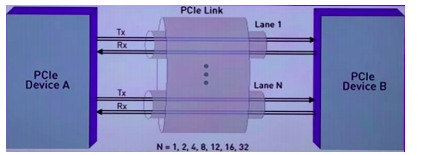
\includegraphics[width=100mm,height=60mm]{images/lane.png}
  \caption{PCIe Link}
  \label{lane}
\end{figure}

In the receiver, PLL circuit (phase locked loop) takes the incoming bit stream as a
reference clock and compares its timing or phase to that of an output clock that it has
created with a specified frequency. Based on the result of that comparison, the output
clock frequency is increased or decreased until a match is obtained, so the output clock
frequency precisely matches the clock that was used to transmit the data. \newline 

Each lane uses differential signaling, this improves noise immunity and reduced signal
voltage. Moreover, anything that will affect the signal will also affect the other by about
the same amount and in the same direction so the receiver won’t be affected by the
noise that affects the signals and will be able to distinguish the bits.

\section{Generations Speeds}

\begin{table}[H]
\caption{PCIe Generations Speeds for link width x16}
    \centering
    \begin{tabular}{|c|c|c|c|}
    \hline
    
    Version & Bandwidth & Gigatransfer & Frequency \\ \hline \hline
         PCIe 1.0  & 8 GB/s & 2.5 GT/s & 2.5 GHz \\ \hline
         PCIe 2.0  & 16 GB/s & 5 GT/s & 5 GHz \\ \hline
         PCIe 3.0  & 32 GB/s & 8 GT/s & 8 GHz \\ \hline
         PCIe 4.0  & 64 GB/s & 16 GT/s & 16 GHz \\ \hline
         PCIe 5.0  & 128 GB/s & 32 GT/s & 32 GHz \\ \hline
        %  PCIe 1.0  & 8 GB/s & 2.5 GT/s & 2.5 GHz \\ \hline
    \end{tabular}

    \label{tab:my_label}
\end{table}
Bandwidth calculations for link width x1:
\begin{equation}
    PCIe_{{B.W}_{Gen1}} = (2.5 Gb/s \times 2 \quad directions)/10 \quad bits \quad per \quad symbol = 0.5 \quad GB/s
\end{equation}
\begin{equation}
    PCIe_{{B.W}_{Gen2}} = (5 Gb/s \times 2 \quad directions)/10 \quad bits \quad per \quad symbol = 1 \quad GB/s
\end{equation}
\begin{equation}
    PCIe_{{B.W}_{Gen3}} = (8 Gb/s \times 2 \quad directions)/8 \quad bits \quad per \quad byte = 1 \quad GB/s
\end{equation}

\section{Topology}

A Topology is composed of point-to-point Links that interconnect a set of components.
This figure \ref{T} illustrates a single fabric instance referred to as a hierarchy – composed of a
Root Complex (RC), multiple Endpoints (I/O devices), a Switch, and a PCI Express to
PCI/PCI-X Bridge, all interconnected via PCI Express Links.
\begin{figure}[H]
  \centering
  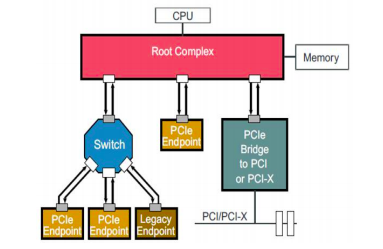
\includegraphics[width=100mm,height=80mm]{images/T.png}
  \caption{Topology}
  \label{T}
\end{figure}

\begin{itemize}
    \item  Root complex: it is the interface between the system CPU and the PCIe topology 
    \begin{itemize}
        \item  Root complex may support one or more PCI Express Ports. Each interface
defines a separate hierarchy domain. Each hierarchy domain may be
composed of a single Endpoint or a sub-hierarchy containing one or more
Switch components and Endpoints.
\item The capability to route peer-to-peer transactions between hierarchy
domains through a Root Complex is optional and implementation
dependent.
    \end{itemize}
    \item Switch: allows more devices to be attached to a single PCIe port, they act as a
packet routers and recognize which path a packet will need to take based on its
address or other routing information (may have several downstream ports but
only one upstream port).
\begin{figure}[H]
  \centering
  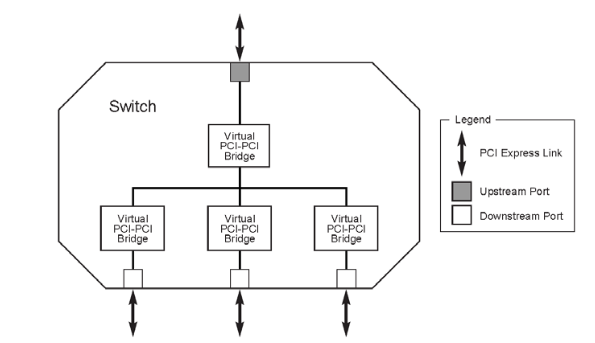
\includegraphics[width=100mm,height=80mm]{images/switch.png}
  \caption{switch}
  \label{lane}
\end{figure}
All Switches are governed by the following base rules:
\begin{itemize}
    \item Switches appear to configuration software as two or more logical PCI-to-PCI Bridges.
    \item Switch must forward all types of Transaction Layer Packets between any
set of Ports.
\item  Switch is not allowed to split a packet into smaller packets.
\end{itemize}
\item Bridge: provides interface to other buses such as PCI or PCI-X or even another
PCIe bus. \newline
Forward bridge $\longrightarrow$ allows older card to be plugged into a new system. \newline
Reverse bridge $\longrightarrow$ allows a new PCIe card to be plugged into an old PCI system.
\item End points: devices that act as initiators and completers of transactions on the
bus (they only implement a single upstream port). Endpoints are classified as
either legacy, PCI Express, or Root Complex Integrated Endpoints.
\end{itemize}
Root complex will appear to configuration software as PCI bus number zero and the PCIe
ports will appear as PCI to PCI bridges. In a similar way, a switch will appear to software
simply as a collection of bridges sharing a common bus. \newline
The advantage of this approach is that it allows the transaction routing to take place in
the same way it did for PCI.
\begin{figure}[H]
  \centering
  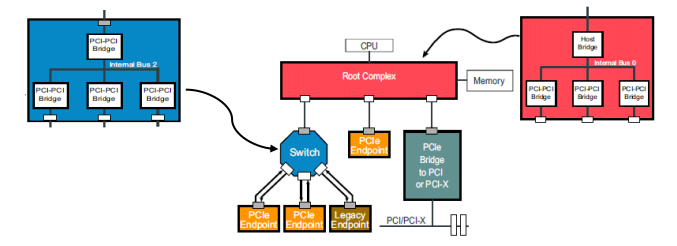
\includegraphics[width=150mm,height=80mm]{images/r.png}
  \caption{configuration software for PCIe}
  \label{fig:r}
\end{figure}

\section{Device layers}
The architecture of PCIe device is divided into three discrete logical layers: Transaction
Layer, Data Link Layer and Physical Layer. Each of these layers is divided into two
sections: one that processes outbound (to be transmitted) information and one that
processes inbound (received) information.
\begin{itemize}
    \item Transaction layer: creation of transaction layer packet (TLP) on the transmit side
and decoding on the receiver side. Also responsible for other 3 functions which
are flow control, quality of service and transaction ordering functionality.
    \item Data link layer: creation of data link layer packet (DLLP) on the transmit side and
decoding on the receiver side. Also, responsible for link error detection and
correction.
    \item Physical layer: creation of ordered set packet on transmit side and decoding on
the receiver side. It processes all 3 types of packets to be transmitted on the link
and processes packets received from the link also. Then packets are encoded and
serialized.
    \item Then link training and status state machine (LTSSM) of the physical layer is
responsible for link initialization and training.

\begin{figure}[H]
  \centering
  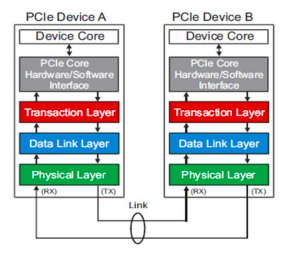
\includegraphics{images/D2.png}
  \caption{Device A and B connect by Link}
  \label{lane}
\end{figure}
    \item Note: switch port needs to implement all the layers as it
evaluates the contents of packets, to determine their
routing requires looking into the internal details of a packet
and that takes place in the transaction layer.

\begin{figure}[H]
  \centering
  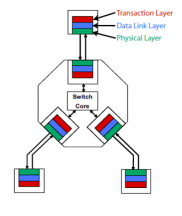
\includegraphics{images/Tl.png}
  \caption{Switch port}
  \label{lane}
\end{figure}
\end{itemize}

\section{layers interaction}
\begin{itemize}
    \item The contents of an outgoing request or completion packet from the device are
assembled in the transaction layer based on information presented by device core
logic. That information would usually include the type of command desired, the
address of the target device and amount of data to transfer.
\item The newly created packet is then stored in a buffer called a virtual channel until it
is ready for passing to the next layer. When the packet is passed down to data link
layer, additional information is added to the packet for error checking at the neighboring receiver and a copy is stored locally so we can send it again if a
transmission error occurs.
\item When the packet arrives at the physical layer, it is encoded and transmitted
differentially using all available lanes of the link.
\item When the packet arrives at the receiver, it decodes the incoming bits in the
physical layer and check for errors that can be seen at this level.
\item if there are no errors, then it forwards the resulting packet up to the data link
layer.
\item Again the resulting packet is checked, if no errors, then it will be forwarded up to
the transaction layer.
\item The packet is buffered, checked for errors and disassembled into the original
information so the contents can be delivered to the device core of the receiver.
\end{itemize}

\section{TLP packet}
\begin{figure}[H]
  \centering
  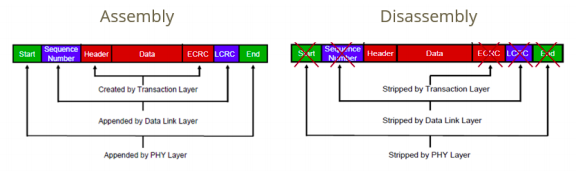
\includegraphics[width=160mm,height=40mm]{images/TLP.png}
  \caption{TLP}
  \label{lane}
\end{figure}
\section{DLLP packet}
They are transferred between data link layers of 2 neighboring devices on a link and the
transaction layer isn’t aware of these packets. Its size is 8 bytes (very small compared to
TLPs).
\begin{figure}[H]
  \centering
  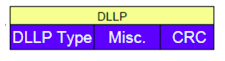
\includegraphics{images/DLLP.png}
  \caption{DLLP}
  \label{lane}
\end{figure}
Note: this DLLP differs from the structure of TLP at the data link layer 

\begin{figure}[H]
  \centering
  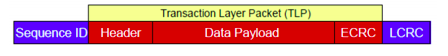
\includegraphics{images/TLP_link_layer.png}
  \caption{TLP at data link layer}
  \label{lane}
\end{figure}

\section{Physical layer}
It is divided into 2 portions:
\begin{enumerate}
    \item Logical $\longrightarrow$  contains the digital logic associated with preparing the packets for
serial transmission on the link and reversing the process for inbound packets.
\item Electrical  $\longrightarrow$ the analog interface that connects to the link and consists of
differential drivers and receivers for each lane.
\end{enumerate}

\begin{figure}[H]
  \centering
  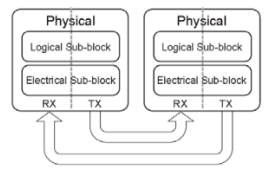
\includegraphics{images/phy.png}
  \caption{Physical Layer}
  \label{lane}
\end{figure}

\section{Logical sub-block}
It has two main sections: Transmit section that prepares outgoing information passed
from the Data Link Layer for transmission by the electrical sub-block, and Receiver
section that identifies and prepares received information before passing it to the Data
Link Layer. The logical sub-block and electrical sub-block coordinate the state of each
Transceiver through a status and control register interface or functional equivalent. The
logical sub-block directs control and management functions of the Physical Layer. PCI
Express uses 8b/10b encoding when the data rate is 2.5 GT/s or 5.0 GT/s. For data rates
greater than or equal to 8.0 GT/s, it uses a per-lane code along with physical layer
encapsulation.\newline \newline 
Logical sub-block contains mainly two logical blocks: MAC layer and PHY.

\section{PIPE Architecture}
\begin{itemize}
    \item Physical Interface for PCI Express Specification (PIPE) developed by Intel, has the
stated intent of providing a standard interface between the internal logic of a
PCIe design and the analog and high-speed circuitry required to implement the
serial link. The purpose of this functional separation is to allow ASIC and
integrated circuit designers to focus on the PCI Express device core, Transaction,
Data Link and logical Physical Layers, while relying on the PIPE-compliant physical
design (PHY) for the electrical interface of the design. 
    \item The PIPE spec defines standard functionality that a PIPE-compliant PHY needs to
implement, as well as a standard parallel interface between the PHY and the
internal logic referred to in the spec as MAC. 

    
\end{itemize}
\begin{figure}[H]
  \centering
  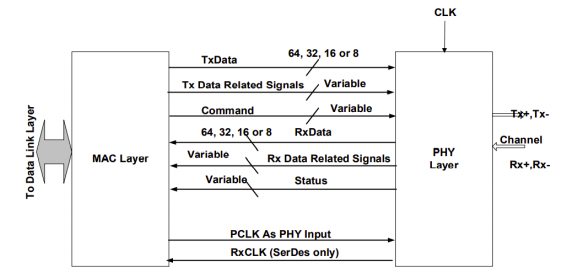
\includegraphics[width=100mm,height=80mm]{images/phymac.png}
  \caption{PHY/MAC Interface}
  \label{lane}
\end{figure}
\subsection{MAC Architecture}

The MAC contains many of the PCIe logical Physical Layer circuits (such as the Link
Training and Status State Machine (LTSSM), data scrambling, byte striping and
functions as the bridge between the DLL and the PHY/MAC interface)
\subsection{PHY/MAC Interface}
It is a parallel interface for transferring data to be transmitted on the PCIe bus.
The width of this parallel interface for bytes of data is shown as either be 8, 16, 32
or 64 bits in each direction.
\subsection{PHY Architecture}
\begin{itemize}
    \item It contains the 8b/10b encoder and decoder, elastic buffer, serializer and deserializer
    \item It contains the logic that controls the receiver detection and reports the detect
status to the MAC via the PHY/MAC Interface.
    \item It contains a Phase Lock Loop (PLL) to generate the internal, high speed clocks
used for the PHY based on the CLK input.
\end{itemize}
\subsection{PIPE PLL}
It generates the PCLK used in synchronizing the parallel PHY/MAC Interface based on the
CLK input.

\begin{figure}[H]
  \centering
  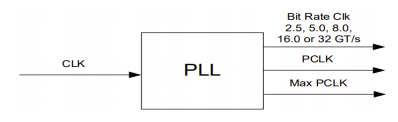
\includegraphics{images/pll.png}
  \caption{PLL}
  \label{lane}
\end{figure}

\subsection{LPIF Architecture}
The LPIF specifications defines common interface between the Link Layer and the logical
physical layer to facilitate interoperability, design and validation re-use between Link
Layers and Physical layers.
\begin{figure}[H]
  \centering
  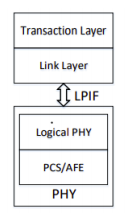
\includegraphics{images/lpif.png}
  \caption{LPIF}
  \label{lane}
\end{figure}

% \begin{figure}[H]
%   \centering
%   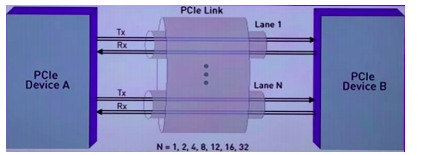
\includegraphics[width=100mm,height=80mm]{images/lane.png}
%   \caption{PCIe Link}
%   \label{lane}
% \end{figure}